\documentclass[a4paper]{article}
\usepackage[left=2.1cm, right=2.1cm, top=2.1cm]{geometry}
\usepackage{lipsum}
\usepackage{tikzpagenodes}
\usepackage{pgfplots}
\usepackage{tikz}
\usepackage{tikz-3dplot}
\usetikzlibrary{arrows,decorations.pathmorphing,backgrounds,positioning,fit,matrix}
\pgfplotsset{compat=1.8}
\usepackage{graphics} % for pdf, bitmapped graphics files
\usepackage{epsfig} % for postscript graphics files
\usepackage[colorlinks=true,citecolor=green]{hyperref}
\usepackage{cite}
\usepackage{amsmath,amssymb,amsfonts}
\usepackage{algorithmic}
\usepackage{graphicx}
\usepackage{url}
\usepackage{cite}
\usepackage{bm}
\usepackage{pbox}
\usepackage{siunitx,booktabs,etoolbox}
\usepackage{ulem}
\usepackage[framed,numbered,autolinebreaks,useliterate]{mcode}
\usepackage{filecontents}
%\usepackage{bigfoot} % to allow verbatim in footnote


\def\BibTeX{{\rm B\kern-.05em{\sc i\kern-.025em b}\kern-.08em
    T\kern-.1667em\lower.7ex\hbox{E}\kern-.125emX}}


\begin{document}

\title{Open project on visual/inertial sensor fusion for image stiching}
\author{xiahaa@space.dtu.dk}
\maketitle%%

In this exercise, you will work (alone) on visual/inertial sensor fusion for image stiching. 

Informally speaking, sensor fusion means you have more than one sensors and there is some mutual (common) information from those sensors that can be fused. For example, sensor A and sensor B both can measure the velocity, then they can fused. Note here measure can be implicit. Recall your assignment in Autonomous Mobile Robots, laser doesn't measure the position directly, but you can infer the position from laser's measurement. So laser can be fused with wheel odometer. If there is no common information, then it is impossible to do sensor fusion. \textbf{This is the principle.}

However, when there is common information, normally there will be more than one way to do the sensor fusion.

I made a trial by computing the relative orientation from images and then fusing the orientation from vision with the orientation from IMU to get a better estimation of the orientation. It can be seen that at least for the figure euler angle (actually, the yaw angle), better result can be obtained. I tried to use this fused orientation to do the image stiching. However, I would say the improvement is limited. 

In stead of following my way of doing sensor fusion, you can try with your own thought or another way in my opinion. I will briefly explain my idea in the following part. 

So another way of doing sensor fusion is inspired by this repository\footnote{\url{https://github.com/yihui-he/panorama}}. In this repository, images are firstly transformed to cylindrical images and then their relationship can be modelled with simple $2$D translation matrices (instead of homography matrices). My idea would be: 1) use vision to compute those translation matrices; 2) use IMU information to compute another set of translation matrices; 3) sensor fusion those translation matrices; 4) use fused matrices to do cylindrical image stiching. 

\textbf{It is up to you to decide whether or not to finish this open project or not since this time, if you choose to do, then you need to do it alone. I can provide you comments and answer you questions, but I will not try to implement this one myself.}

\begin{figure}[!b]
\centering
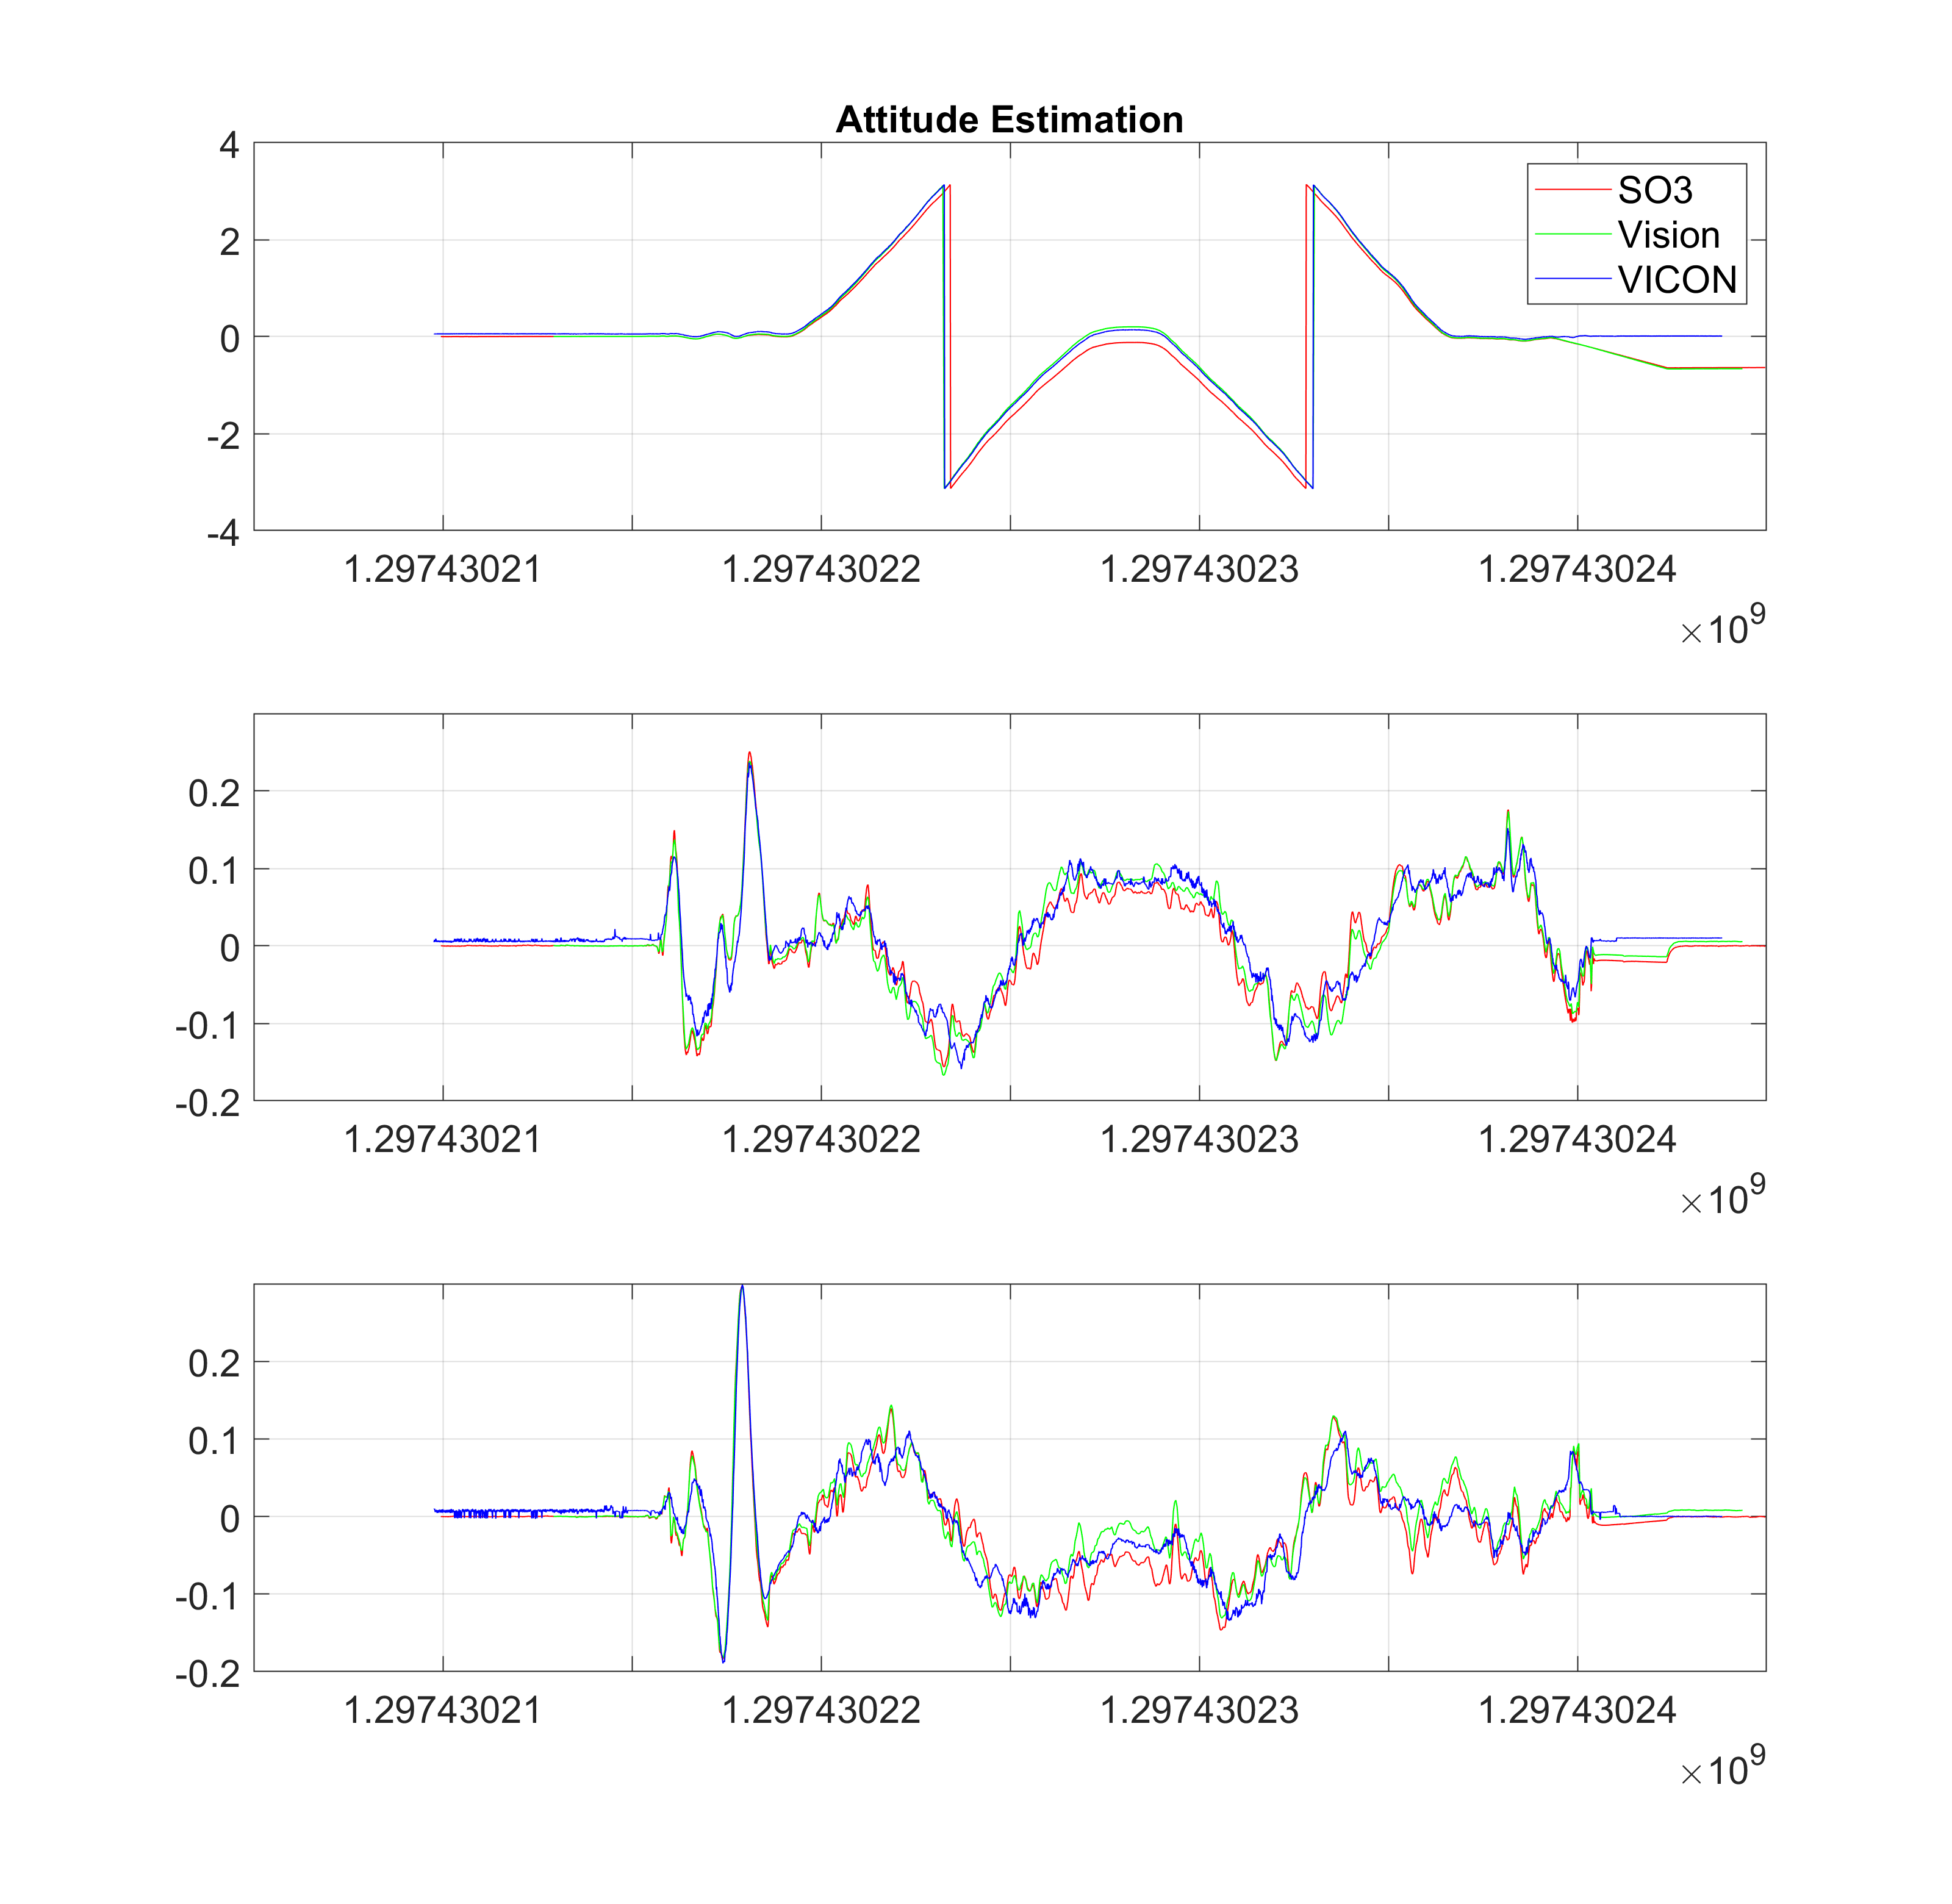
\includegraphics[scale=0.3]{figures/so3_2.png}
\end{figure}

\end{document}